\documentclass[10pt]{article}

% Lines beginning with the percent sign are comments
% This file has been commented to help you understand more about LaTeX

% DO NOT EDIT THE LINES BETWEEN THE TWO LONG HORIZONTAL LINES

%---------------------------------------------------------------------------------------------------------

% Packages add extra functionality.
\usepackage{times,graphicx,epstopdf,fancyhdr,amsfonts,amsthm,amsmath,algorithm,algorithmic,xspace,hyperref}
\usepackage[left=1in,top=1in,right=1in,bottom=1in]{geometry}
\usepackage{sect sty}	%For centering section headings
\usepackage{enumerate}	%Allows more labeling options for enumerate environments 
\usepackage{epsfig}
\usepackage[space]{grffile}
\usepackage{booktabs}
\usepackage{forest}
\usepackage{enumitem}   
\usepackage{fancyvrb}
\usepackage{todonotes}
\usepackage{setspace}
\usepackage{multirow}


% This will set LaTeX to look for figures in the same directory as the .tex file
\graphicspath{.} % The dot means current directory.

\pagestyle{fancy}

\lhead{Final Project}
\rhead{\today}
\lfoot{CSCI 334: Principles of Programming Languages}
\cfoot{\thepage}
\rfoot{Spring 2024}

% Some commands for changing header and footer format
\renewcommand{\headrulewidth}{0.4pt}
\renewcommand{\headwidth}{\textwidth}
\renewcommand{\footrulewidth}{0.4pt}

% These let you use common environments
\newtheorem{claim}{Claim}
\newtheorem{definition}{Definition}
\newtheorem{theorem}{Theorem}
\newtheorem{lemma}{Lemma}
\newtheorem{observation}{Observation}
\newtheorem{question}{Question}

\setlength{\parindent}{0cm}

%---------------------------------------------------------------------------------------------------------

% DON'T CHANGE ANYTHING ABOVE HERE

% Edit below as instructed

\title{Twined Language Specification} % Replace SnappyLanguageName with your project's name

\author{Lucas Weissman \and Zach Sturdevant} % Replace these with real partner names.

\begin{document}
  
\maketitle

\subsection*{Introduction}

  \begin{spacing}{1.2}
    \hspace*{1cm} "Twined" is a knowledge programming language that aims to revolutionize the way
    we manage and interact with textual information. By converting unstructured text
    data into structured, navigable knowledge graphs, "Twined" enhances comprehension
    and analysis, providing a unique interactive interface that allows users to 
    explore information and create insights through based reasoning visualizations.
    \end{spacing}
  \singlespacing

  \begin{spacing}{1.2}
  "Twined" addresses the problem of inefficient management and interaction with the 
  ever-growing volume of new information one can retain, making it a powerful tool
  for researchers, analysts, students, and anyone who works with text-based 
  information and wants to uncover hidden connections, identify patterns, and
  derive meaningful conclusions. By providing a platform that encourages 
  exploration, critical thinking, and the synthesis of ideas from various fields, 
  "Twined" aims to replicate the transformative learning experience offered by 
  liberal arts institutions by promoting users to twine the
  threads of information into their own personal tapestry of knowledge.
  \end{spacing}

\subsection*{Design Principles}

  \begin{spacing}{1.2}
    \hspace*{1cm} The design of "Twined" is guided by both aesthetic and technical ideas that aim
    to make knowledge more accessible and manageable for users. From an aesthetic
    standpoint, the language strives to provide a simple and intuitive starting
    point that gradually evolves into a powerful graphical user interface. This
    approach ensures that users of all skill levels can easily interact with 
    the language and leverage its capabilities without being overwhelmed by
    complexity. By prioritizing user experience and usability, "Twined" aims to
    create an engaging and visually appealing environment that encourages exploration
    and discovery. 
  \end{spacing}

  \begin{spacing}{1.2}
  From a technical perspective, "Twined" uses the power of generative AI to
  enhance the efficiency and effectiveness of knowledge access and management.
  The language aims to minimize user input while maximizing the usefulness
  of the output, allowing users to obtain valuable insights and connections
  with minimal effort. As the language evolves, it will incorporate features 
  that enable users to upload text and express their desired outcomes
  in natural language. "Twined" will then handle customized outputs
  to the user.
  \end{spacing}

\newpage
  \subsection*{Examples}
    \begin{enumerate}
      \item 
        \begin{enumerate}
          \item Program 1 input
            \begin{verbatim}
              {Nancy, (Fred, Sally, Sarah,)}
              {Fred, (Nancy, Sally, Sarah,)}
              {Sally, (Jeff, Jonny, Timmy,)}
              {Jeff, (Sally, Jonny, Timmy,)}
            \end{verbatim}
          \item Program 1 output
            \begin{figure}[!hb]
              \centering
              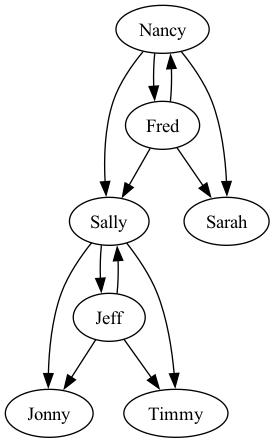
\includegraphics[width=0.3\linewidth]{images/family_tree.png} 
              \caption{Family Relationship}
              \label{figure 1:}
            \end{figure}
          \item
            This graph represents the relationships between family individuals. Each node represents 
            a person, and each edge represents a direct relationship between two individuals. For example,
            "Nancy" has relationships with "Sally," "Fred," and "Sarah," as depicted by the edges 
            connecting their respective nodes.
        \end{enumerate}
      
      \item
        \begin{enumerate}
          \item Program 2 input
            \begin{verbatim}
              {Sunlight, (PlantGrowth,)}
              {Water, (PlantGrowth,)}
              {SoilNutrients, (PlantGrowth,)}
            \end{verbatim}
          \item Program 2 output
            \begin{figure}[!hb]
              \centering
              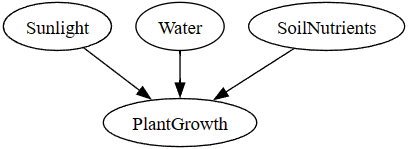
\includegraphics[width=0.4\linewidth]{images/plant_test_0.1.png} 
              \caption{Plant Growth Relationship}
              \label{figure 2:}
            \end{figure}
          \item
            The graph represents factors affecting plant growth. Each node represents
            a factor such as "Sunlight," "Water," and "Soil Nutrients," and each edge 
            represents the influence of these factors on "Plant Growth," as depicted 
            by the edges connecting their respective nodes.
        \end{enumerate}
        
      \item
        \begin{enumerate}
          \item Program 3 input
            \begin{verbatim}
              {European Fascism, (Germany, Italy, Spain,)}
              {Germany, (Adolf Hitler,)}
              {Italy, (Benito Mussolini,)}
              {Spain,(Francisco Franco,)}
            \end{verbatim}
          \item Program 3 output
            \begin{figure}[!hb]
              \centering
              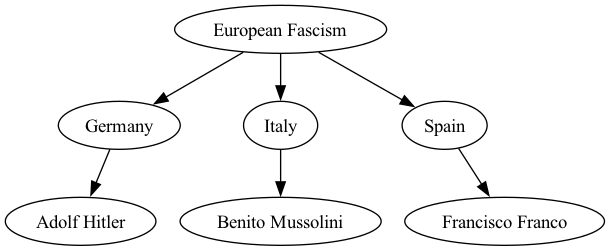
\includegraphics[width=0.5\linewidth]{images/Fascism.png} 
              \caption{Famious Eureopean Fascists}
              \label{figure 3:}
            \end{figure}
          \item
            This graph shows connections between European Fascism and leaders 
            of different Fascist countries. Each node represents a topic and 
            how those topics are connected in a top down manner.
            
        \end{enumerate}
    \end{enumerate}


\newpage
\subsection*{Language Concepts}
    \begin{spacing}{1.2}
      \hspace*{1cm} To effectively use "Twined," users should understand the fundamental concepts of
      knowledge graphs and how they represent information. While the language aims to
      minimize the need for users to grasp low-level primitives, a basic understanding
      of nodes and edges is still beneficial. Nodes represent entities or concepts 
      within the text, while edges signify the relationships or connections between 
      them. These concepts enables "Twined" to create dynamic interactive knowledge graphs 
      that highlight both hierarchical and associative relationships. By comprehending 
      how these elements interact, users can better navigate and interpret the visual 
      representation of their data. 

      \singlespacing
      "Twined" will provide an intuitive and user-friendly experience through an interface,
      for inputting their desired information to explore knowledge graphs. The user interface 
      will offer tools for navigating the graph, filtering information, and discovering new
      connections.
    \end{spacing}

  \subsection*{Formal Syntax}
    \singlespacing
      \begin{tabular}{lll}
          $<\textbf{expression}>$ & ::= & $<\textbf{Node}>$  \\
                                  & $|$  & $<\textbf{edgeList}>$ \\
                                  & $|$  & $<\textbf{nodeName}>$ \\
                                  & $|$  & $<\textbf{listOfNodes}>$ \\
                                  
          $<\textbf{Node}>$   & ::= & \{ $<\textbf{String}>$, $<\textbf{nodeName}>$ \} \\
          $<\textbf{nodeName}>$& ::= &  $<\textbf{String}>$ \\
          $<\textbf{edgeList}>$& ::= & ($<\textbf{nodeName}>$ +) \\
          $<\textbf{listOfNodes}>$& ::= & $<\textbf{Node}>$ + \\
          
          \end{tabular}

\subsection*{Semantics}

  \begin{table}[h!]
    \begin{center}
      %\caption{Multirow table.}
      \label{tab:table1}
      \begin{tabular}{l|c|r|l}
        \textbf{Syntax} & \textbf{Abstract Syntax} & \textbf{Prec./Assoc.} & \textbf{Meaning}\\
        \hline
        $<$\text{NodeName}$>$ & Name of string & N/A & NodeName is a primative\\
        & & & represented using an f\# string\\
        
        \hline
        $<$\text{EdgeList}$>$ & NodeName list & N/A & An edgeList is a list of\\
        & & &  NodeNames stored in an f\# list\\
        \hline
        $<$\text{Node}$>$ & Node of (NodeName * EdgeList) & N/A & A node is a combining form\\
        & & & that stores a NodeName and \\
        & & & a list of nodes that that node is\\
        & & & connected to in an f\# list \\
        \hline
        $<$\text{NodeList}$>$ & Node list & N/A &A series of nodes in the form\\
        & & & \{node\} \{node\}\\
        & & & separated by whitespace including\\ 
        & & & newlines these are used to store all \\
        & & & nodes in a graph\\
        \hline
        $<$\text{NodeInfo}$>$& NodeInfo of String & N/A & primative of information that will\\
        & & &  be associated with a node\\
        & & & represented with an f\# string.\\
        
        \hline
        $<$\text{NodeName}$>$ := $<$\text{NodeInfo}$>$& Definition of NodeName := NodeInfo & N/A & A node is a combining form that\\
        & & & stores a NodeName and a list of \\
        & & & nodes that the named node is \\
        & & &  connected to in an f\# list \\

      \end{tabular}
    \end{center}
  \end{table}

    \begin{enumerate}
      \item Primitive values:
        \begin{enumerate}
          \item NodeName: A series of characters digits or spaces that represent the name of a node. stored in
          a string.
          \item EdgeList: A series of NodeNames, or 0 stored in the form (NodeName, NodeName,) 
          that contains the NodeNames of nodes connected to the node, stored in a list.
        \end{enumerate}
      \item Combining forms:
        \begin{enumerate}
          \item Node: A tuple of the form {NodeName, (EdgeList)} that represents a full node, which is
          the name of the node and its EdgeList. In the future the node name will be used to access
          a dictionary that contains the information associted with that node
          \item NodeList: A series of nodes in the form Node Node separated by whitespace including newlines
          these are used to represent all nodes in a graph
        \end{enumerate}
      \item Evalutation:
          \begin{enumerate}
            \item The programs in our language read inputs given in a txt file, it parses the text file and
            separating the series of nodes and their edges.
            \item When the program is evaluated it produces a graph using the nodes and their edgelist on the
            screen
          \end{enumerate}
    \end{enumerate}

\newpage
\begin{figure} 
  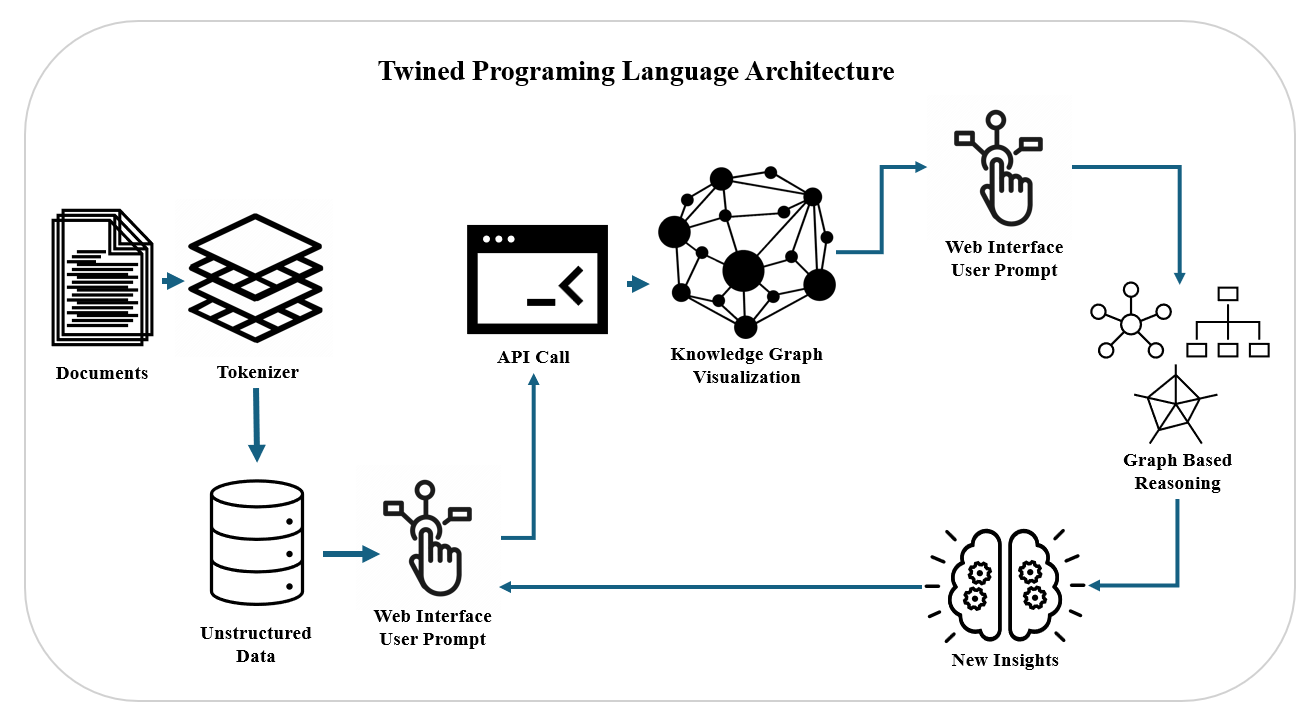
\includegraphics[width=1\linewidth]{images/ArchitectureDiagram.png} 
\end{figure}
% DO NOT DELETE ANYTHING BELOW THIS LINE
\end{document}
